\documentclass{article}
\usepackage{graphicx}
\usepackage{listings}
\usepackage{enumitem}
\title{Minimax vs Reinforcement Learning}
\author{Vijaya Sinha \and Shayan DasGupta \and Sudipta Maity}

\begin{document}
\maketitle

\newpage
\section{Introduction}

Artificial Intelligence (AI) algorithms have made significant advancements in various domains, prompting curiosity about how different algorithms perform when compared against each other. In this research, we explore the performance of two prominent AI approaches, Minimax and Reinforcement Learning (RL), by pitting them against each other in games such as Tic-Tac-Toe, Connect Four, and Chess.

Minimax, a classic algorithm for two-player, zero-sum games, employs a game tree to consider all possible moves. It aims to minimize the maximum potential loss, assuming optimal play by the opponent. In contrast, RL is a paradigm that enables agents to learn optimal behavior through interaction with their environment. Agents use trial and error to maximize a reward signal, updating their policies accordingly.

To evaluate and compare the performance of Minimax and RL, we selected Tic-Tac-Toe, Connect Four, and Chess as our testbed games. Each game offers distinct characteristics in terms of complexity, strategic depth, and the number of possible moves. Tic-Tac-Toe represents a simple game with limited moves, while Connect Four presents a larger decision space. Chess, known for its complexity and vast number of positions, serves as a challenging benchmark.

Through this research, we aim to gain insights into the strengths and weaknesses of Minimax and RL algorithms. We anticipate that Minimax will excel in games with smaller state spaces, relying on strategic planning and foresight. In contrast, RL algorithms are expected to demonstrate adaptability and better performance in games with larger state spaces, emphasizing exploration and exploitation.

This report outlines our experiment's methodology, the setup used, the obtained results, and subsequent discussions. Additionally, we explore potential avenues for future work that can further enhance the understanding and application of these AI algorithms in game-playing scenarios.

\newpage

\section{Methodology}
In this section, we describe the methodology employed for conducting the experiments and comparing the performance of Minimax and Q-learning algorithms in different games: Tic-Tac-Toe, Connect Four, and Chess. Specifically, we investigate the following scenarios:

\subsection{Tic-Tac-Toe}
To assess the performance of Minimax and Q-learning in Tic-Tac-Toe, we conducted three sets of experiments:

1.1 \textbf{Minimax vs Q-learning}: We implemented Minimax and Q-learning algorithms to play against each other in multiple games of Tic-Tac-Toe. We recorded the outcomes and evaluated their relative performance based on win rates and game completion time.

1.2 \textbf{Minimax vs Random Agent}: We introduced a random agent as an opponent to Minimax. The random agent made random moves without any strategic planning or learning. We compared the performance of Minimax against the random agent and recorded the results to analyze the effectiveness of Minimax's strategic planning in a competitive setting.

1.3 \textbf{Q-learning vs Random Agent}: Similarly, we made Q-learning play against the random agent to assess its performance in the absence of strategic planning. The results were recorded and analyzed to understand the adaptability and learning capabilities of the Q-learning algorithm.


\subsection{Connect Four}
For the game of Connect Four, we followed a similar approach and conducted the following experiments:

2.1 \textbf{Minimax vs Q-learning}: We implemented both Minimax and Q-learning algorithms to compete against each other in multiple games of Connect Four. The results were recorded and compared to evaluate the strengths and weaknesses of the algorithms in this game.

2.2 \textbf{Minimax vs Random Agent}: We introduced a random agent as an opponent to Minimax and evaluated its performance against the random agent in Connect Four. The objective was to understand how Minimax's strategic planning fared against a non-learning, random player.

2.3 \textbf{Q-learning vs Random Agent}: Similarly, we made Q-learning play against the random agent to measure its adaptability and ability to learn in the game of Connect Four. The performance of Q-learning was compared against the random agent to assess its effectiveness.

\pagebreak
\subsection{Chess}
Lastly, we explored the performance of Minimax and Q-learning in the highly complex game of Chess:

3.1 \textbf{Minimax vs Q-learning}: We implemented Minimax and Q-learning algorithms to play against each other in a series of Chess games. The outcomes were recorded and analyzed to determine the relative performance of the algorithms in this challenging domain.

3.2 \textbf{Minimax vs Random Agent}: We introduced a random agent as an opponent to Minimax and evaluated its performance against the random agent in Chess. This comparison aimed to assess the strategic planning and decision-making capabilities of Minimax in a complex game like Chess.

3.3 \textbf{Q-learning vs Random Agent}: Lastly, we made Q-learning play against the random agent in Chess to evaluate its adaptability and learning capabilities. The performance of Q-learning against the random agent was measured and analyzed to understand its effectiveness in Chess.

The results from these experiments were meticulously recorded, and the performance of Minimax, Q-learning, and the random agent was compared and analyzed for each game. The subsequent sections of this report will present and discuss these findings in detail.

\pagebreak
\section{Code Implementation}

\subsection{Tic Tac Toe}

\subsubsection{Minimax vs Q-Learning}
\begin{enumerate}
  \item Tic Tac Toe Game Implementation:
    \begin{itemize}
      \item The \texttt{TicTacToe} class represents the Tic Tac Toe game.
      \item The \texttt{\_\_init\_\_} method initializes the game board and the current player.
      \item The \texttt{display\_board} method prints the current state of the game board.
      \item The \texttt{make\_move} method updates the game board with a player's move.
      \item The \texttt{is\_winner} method checks if a player has won the game.
      \item The \texttt{is\_draw} method checks if the game is a draw.
      \item The \texttt{is\_game\_over} method checks if the game is over (win, draw, or ongoing).
    \end{itemize}

  \item Minimax Player Implementation:
    \begin{itemize}
      \item The \texttt{MinimaxPlayer} class represents a player that uses the Minimax algorithm to make moves.
      \item The \texttt{get\_best\_move} method calculates the best move using the Minimax algorithm.
      \item The \texttt{minimax} method recursively evaluates all possible moves to determine the best score.
    \end{itemize}

  \item Q-learning Player Implementation:
    \begin{itemize}
      \item The \texttt{QLearningPlayer} class represents a player that uses Q-learning to make moves.
      \item The \texttt{get\_best\_move} method selects the best move using the Q-learning strategy.
      \item The \texttt{update\_q\_table} method updates the Q-table based on the current state, action, next state, and reward.
    \end{itemize}

  \item \texttt{play\_game} Function:
    \begin{itemize}
      \item The \texttt{play\_game} function simulates a game between two players.
      \item It alternates the turns between the players until the game is over.
      \item It calls the appropriate methods of the players to make moves and update the Q-table.
    \end{itemize}

  \item Main Program:
    \begin{itemize}
      \item The main program initializes a Minimax player (\texttt{player1}) and a Q-learning player (\texttt{player2}).
      \item It tracks the number of games won by each player.
      \item It plays a specified number of games (200 in this case) between the two players.
      \item After each game, it prints the game board and updates the win records.
      \item Finally, it displays the number of games won by each player and the win records for each game.
    \end{itemize}
\end{enumerate}
\begin{figure}[htbp]
    \centering
    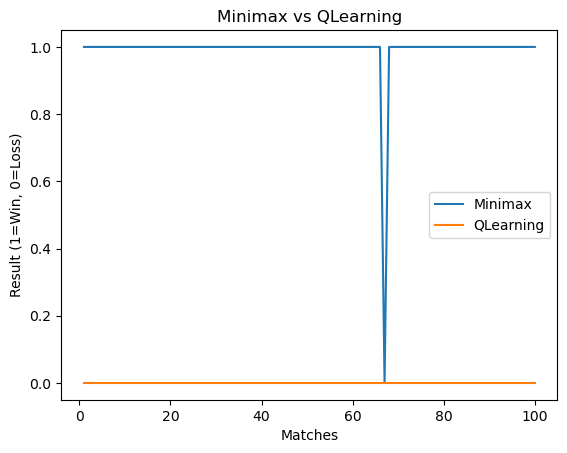
\includegraphics[width=0.6\textwidth]{img 1.png}
    \caption{Minimax vs QLearning}
    \label{fig:example}
\end{figure}


\subsubsection{Minimax vs Random Agent and  Q-Learning vs Random Agent}
\begin{enumerate}
  \item TicTacToe Class:
    \begin{itemize}
      \item Initializes the game board and the current player.
      \item Provides a method to display the current state of the board.
      \item Allows making a move on the board.
      \item Checks if a player has won the game.
      \item Checks if the game is a draw.
      \item Checks if the game is over (either a player has won or it's a draw).
    \end{itemize}

  \item MinimaxPlayer Class:
    \begin{itemize}
      \item Takes a player ('X' or 'O') as input.
      \item Implements the minimax algorithm to determine the best move for the player.
      \item Uses recursion to explore all possible moves and outcomes of the game.
      \item Returns the best move based on the calculated scores.
    \end{itemize}

  \item QLearningPlayer Class:
    \begin{itemize}
      \item Takes a player ('X' or 'O') and several parameters (learning rate, discount factor, exploration rate) as input.
      \item Maintains a Q-table to store the estimated Q-values for state-action pairs.
      \item Implements the epsilon-greedy exploration-exploitation strategy.
      \item Provides a method to update the Q-table based on rewards and the observed next state.
      \item Decreases the exploration rate over time.
      \item Returns the best move based on the Q-values in the Q-table.
    \end{itemize}

  \item RandomAgent Class:
    \begin{itemize}
      \item Implements a simple agent that selects a random move from the available legal moves.
    \end{itemize}

  \item \texttt{play\_game()} Function:
    \begin{itemize}
      \item Takes two players as input and plays a complete Tic Tac Toe game between them.
      \item Alternates the current player's turn until the game is over.
      \item If the current player is a QLearningPlayer, updates the Q-table based on the observed rewards and states.
    \end{itemize}

  \item \texttt{play\_game\_vs\_random()} Function:
    \begin{itemize}
      \item Takes a player and a random agent as input and plays a complete Tic Tac Toe game between them.
      \item Alternates the current player's turn until the game is over.
      \item Returns the final game state.
    \end{itemize}

  \item Main Program:
    \begin{itemize}
      \item Creates instances of MinimaxPlayer, RandomAgent, and QLearningPlayer.
      \item Plays 100 games of MinimaxPlayer against RandomAgent and keeps track of the results.
      \item Plays 100 games of QLearningPlayer against RandomAgent and keeps track of the results.
      \item Prints the results, including the number of games won and drawn by each player.
    \end{itemize}
\end{enumerate}
\begin{figure}[htbp]
    \centering
    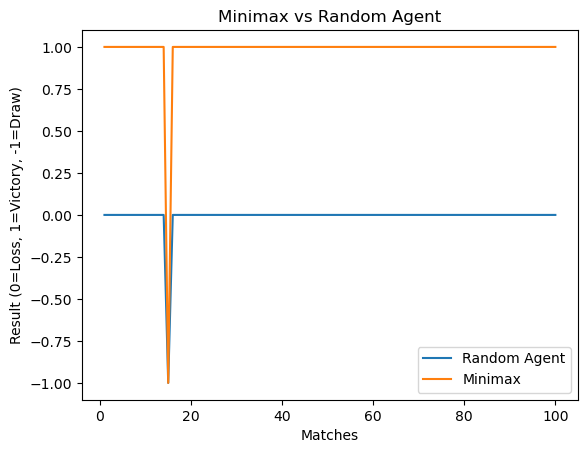
\includegraphics[width=0.9\textwidth]{img 2.png}
    \caption{Minimax vs Random Agent}
    \label{fig:example}
\end{figure}
\begin{figure}[htbp]
    \centering
    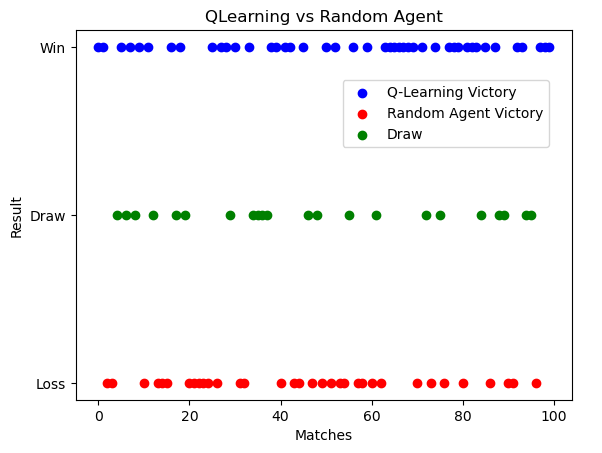
\includegraphics[width=0.9\textwidth]{img 3.png}
    \caption{QLearning vs Random Agent}
    \label{fig:example}
\end{figure}


\subsection{Connect Four}

\subsubsection{Minimax vs Q-Learning}
\begin{enumerate}
    \item \texttt{\_\_init\_\_} function initializes the MiniMax class and sets the maximum depth and player symbol.
    \item \texttt{choose\_move} function selects the best move using the MiniMax algorithm with alpha-beta pruning.
    \item \texttt{minmax} function implements the MiniMax algorithm recursively, considering different moves and evaluating board states.
    \item \texttt{evaluate\_board} function evaluates the score of the board for the given player symbol.
    \item \texttt{evaluate\_window} function evaluates the score of a window of four cells on the board for the given player symbol.
\end{enumerate}

\begin{enumerate}
    \item \texttt{\_\_init\_\_} function initializes the QLearning class and sets the symbol, learning rate, discount factor, exploration factor, and Q-table.
    \item \texttt{state\_to\_string} function converts the board state to a string representation.
    \item \texttt{choose\_move} function selects the best move based on the current board state and the Q-table values, using an exploration-exploitation strategy.
    \item \texttt{update\_q\_table} function updates the Q-table based on the current state, action, next state, and reward.
\end{enumerate}
\begin{enumerate}
    \item \texttt{\_\_init\_\_} function initializes the ConnectFour class and sets up the board, player symbols, and move lists.
    \item \texttt{is\_valid\_move} function checks if a move is valid on the given board.
    \item \texttt{do\_move} function makes a move on the board and updates the move lists.
    \item \texttt{undo\_move} function undoes a move on the board and updates the move lists.
    \item \texttt{is\_winner} function checks if a player has won the game on the given board.
    \item \texttt{is\_draw} function checks if the game is a draw on the given board.
    \item \texttt{moves\_available} function checks if there are any moves available on the given board.
    \item \texttt{refresh\_board} function resets the board and move lists.
\end{enumerate}
\begin{enumerate}
    \item The \texttt{main} function is the entry point of the program.
    \item The function sets up the game board, creates instances of the QLearning and MiniMax classes, and initializes scores.
    \item The function runs a loop for a specified number of episodes, where each episode represents a game.
    \item Within each episode, the game board is refreshed, and the players take turns choosing moves until the game is won or drawn.
    \item The QLearning player updates its Q-table based on the outcome of the game.
    \item After the episodes, the function prints the scores and displays a plot comparing the scores of QLearning and MiniMax players.
\end{enumerate}
\begin{figure}[htbp]
    \centering
    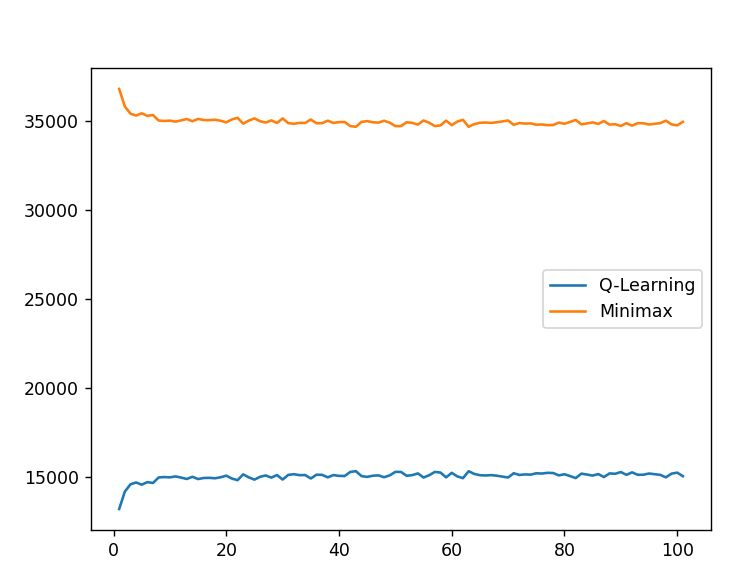
\includegraphics[width=0.9\textwidth]{img 4.jpg}
    \caption{Minimax vs Random Agent}
    \label{fig:example}
\end{figure}


\subsubsection{Minimax vs Random Agent and  Q-Learning vs Random Agent}

\begin{enumerate}
  \item \texttt{QNetwork} class: Defines a neural network model for Q-learning.
  \item \texttt{\_\_init\_\_} method: Initializes the \texttt{QNetwork} class with input and output sizes.
  \item \texttt{forward} method: Performs forward pass computations of the neural network.
  \item \texttt{QLearning} class: Implements the Q-learning algorithm.
  \item \texttt{\_\_init\_\_} method: Initializes the \texttt{QLearning} class with learning parameters and creates a QNetwork instance.
  \item \texttt{choose\_move} method: Chooses a move based on the current state and the Q-network's predictions.
  \item \texttt{update\_q\_table} method: Updates the Q-table based on the current state, action, next state, and reward.
  \item \texttt{preprocess\_state} method: Preprocesses the game board state for input to the neural network.
  \item \texttt{train} method: Trains the Q-learning agent using the given game board and a specified number of episodes.
  \item \texttt{MiniMax} class: Implements the minimax algorithm for move selection.
  \item \texttt{\_\_init\_\_} method: Initializes the \texttt{MiniMax} class with maximum depth and player symbol.
  \item \texttt{choose\_move} method: Chooses the best move using the minimax algorithm.
  \item \texttt{minmax} method: Performs the minimax algorithm for evaluating game states and selecting moves.
  \item \texttt{evaluate\_board} method: Evaluates the score of a game board state for a given player symbol.
  \item \texttt{evaluate\_window} method: Evaluates the score of a window of cells in a game board.
  \item \texttt{ConnectFour} class: Implements the game logic for Connect Four.
  \item \texttt{\_\_init\_\_} method: Initializes the \texttt{ConnectFour} class with an empty game board.
  \item \texttt{is\_valid\_move} method: Checks if a move is valid on the game board.
  \item \texttt{do\_move} method: Performs a move on the game board.
  \item \texttt{undo\_move} method: Undoes a move on the game board.
  \item \texttt{is\_winner} method: Checks if a player has won the game.
  \item \texttt{is\_draw} method: Checks if the game is a draw.
  \item \texttt{moves\_available} method: Checks if there are any available moves on the game board.
  \item \texttt{refresh\_board} method: Refreshes the game board to an empty state.
  \item \texttt{main} function: Implements the main game loop and evaluates the performance of different players.
\end{enumerate}
\begin{figure}[htbp]
    \centering
    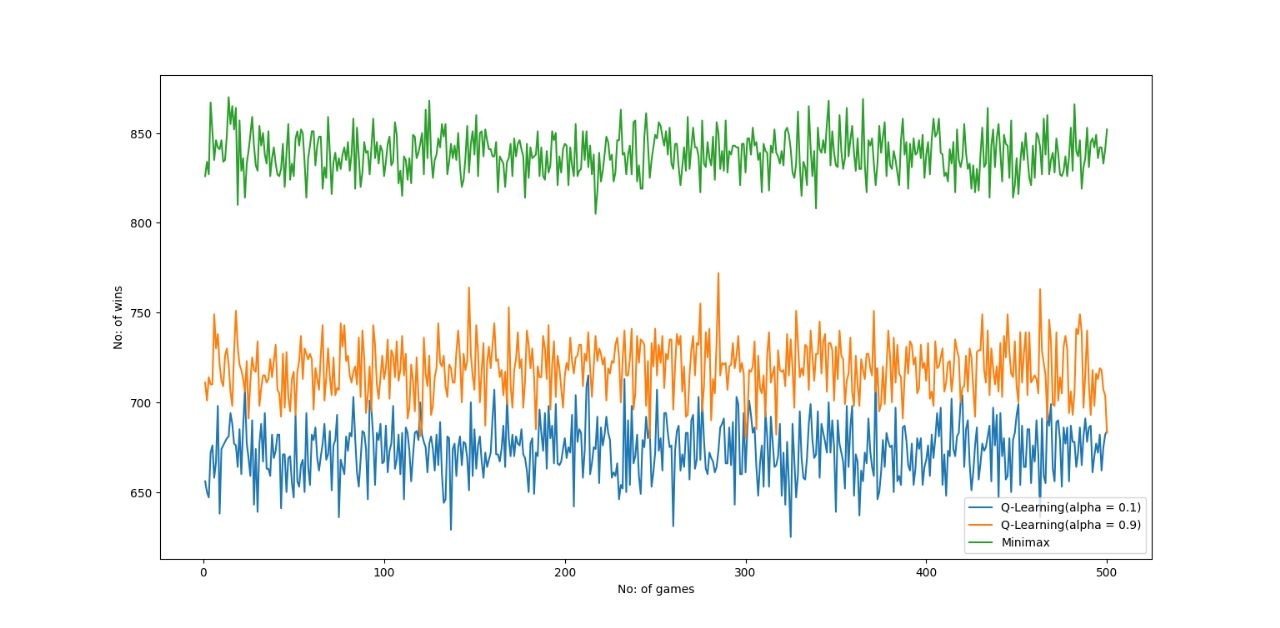
\includegraphics[width=1.2\textwidth]{img 56.jpg}
    \caption{Minimax vs Random Agent}
    \label{fig:example}
\end{figure}


\subsection{Chess}

\subsubsection{Minimax vs Q-Learning}

\begin{enumerate}
  \item \texttt{ChessGame} class:
    \begin{itemize}
      \item \texttt{\_\_init\_\_()}: Initializes a new chess game with a chess board.
      \item \texttt{initialize\_game()}: Resets the chess board to the initial position.
      \item \texttt{get\_board()}: Returns a copy of the current chess board.
      \item \texttt{get\_current\_player()}: Returns the current player in the game.
      \item \texttt{make\_move(move)}: Makes a move on the chess board if it is a legal move.
      \item \texttt{is\_game\_over()}: Checks if the game is over (e.g., checkmate or stalemate).
    \end{itemize}
    
  \item \texttt{QLearningAgent} class:
    \begin{itemize}
      \item \texttt{\_\_init\_\_(state\_size, action\_size, learning\_rate, discount\_factor, exploration\_rate, exploration\_decay)}: Initializes a Q-learning agent with the given parameters.
      \item \texttt{choose\_action(state)}: Chooses an action to take based on the current state and exploration rate.
      \item \texttt{get\_best\_action(state)}: Returns the best action to take in the given state based on the Q-table.
      \item \texttt{update\_q\_table(state, action, reward, next\_state)}: Updates the Q-table based on the observed state, action, reward, and next state.
      \item \texttt{decay\_exploration\_rate()}: Decays the exploration rate over time to encourage exploitation.
      \item \texttt{get\_q\_table()}: Returns the current Q-table.
    \end{itemize}
    
  \item \texttt{convert\_board\_to\_state(board)} function: Converts the current chess board to a state representation that can be used by the Q-learning agent.
  
  \item \texttt{MinimaxAgent} class:
    \begin{itemize}
      \item \texttt{\_\_init\_\_(max\_depth)}: Initializes a minimax agent with the given maximum search depth.
      \item \texttt{choose\_move(board)}: Chooses the best move to make on the chess board using the minimax algorithm.
      \item \texttt{evaluate\_board(board)}: Evaluates the current chess board and returns a score indicating the advantage of the white player.
      \item \texttt{minimax(board, depth, alpha, beta, maximizing\_player)}: Implements the minimax algorithm with alpha-beta pruning to determine the optimal move for the current player.
    \end{itemize}
    
  \item \texttt{Main} class:
    \begin{itemize}
      \item \texttt{\_\_init\_\_(num\_episodes, max\_depth)}: Initializes the main class with the number of episodes and maximum search depth.
      \item \texttt{play\_game()}: Plays the chess game for the specified number of episodes using Q-learning and minimax agents.
    \end{itemize}
  
  \item Additional variables:
    \begin{itemize}
      \item \texttt{num\_episodes}: The number of episodes to train the Q-learning agent.
      \item \texttt{max\_depth}: The maximum search depth for the minimax agent.
    \end{itemize}
\end{enumerate}
\begin{figure}[htbp]
    \centering
    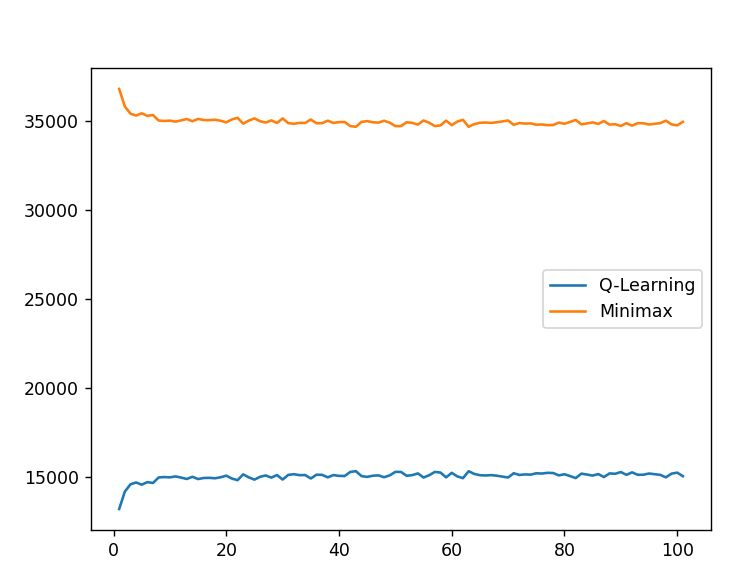
\includegraphics[width=0.9\textwidth]{img 4.jpg}
    \caption{Minimax vs Random Agent}
    \label{fig:example}
\end{figure}

\subsubsection{Minimax vs Random Agent and  Q-Learning vs Random Agent}
\begin{enumerate}
  \item \texttt{ChessGame} class:
    \begin{itemize}
      \item \texttt{\_\_init\_\_()}: Initializes a new chess game with a chess board.
      \item \texttt{initialize\_game()}: Resets the chess board to the initial position.
      \item \texttt{get\_board()}: Returns a copy of the current chess board.
      \item \texttt{get\_current\_player()}: Returns the current player in the game.
      \item \texttt{make\_move(move)}: Makes a move on the chess board if it is a legal move.
      \item \texttt{is\_game\_over()}: Checks if the game is over.
    \end{itemize}

  \item \texttt{QLearningAgent} class:
    \begin{itemize}
      \item \texttt{\_\_init\_\_(state\_size, action\_size, learning\_rate, discount\_factor, exploration\_rate, exploration\_decay)}: Initializes a Q-learning agent with the given parameters.
      \item \texttt{choose\_action(state)}: Chooses an action to take based on the current state and exploration rate.
      \item \texttt{get\_best\_action(state)}: Returns the best action to take in the given state based on the Q-table.
      \item \texttt{update\_q\_table(state, action, reward, next\_state)}: Updates the Q-table based on the observed state, action, reward, and next state.
      \item \texttt{decay\_exploration\_rate()}: Decays the exploration rate over time.
      \item \texttt{get\_q\_table()}: Returns the current Q-table.
    \end{itemize}

  \item \texttt{RandomAgent} class:
    \begin{itemize}
      \item \texttt{\_\_init\_\_()}: Initializes a random agent.
      \item \texttt{choose\_move(board)}: Chooses a random move from the legal moves on the chess board.
    \end{itemize}

  \item \texttt{Main} class:
    \begin{itemize}
      \item \texttt{\_\_init\_\_(num\_episodes)}: Initializes the main class with the number of episodes.
      \item \texttt{play\_game()}: Plays the chess game for the specified number of episodes using the Q-learning and random agents.
      \item \texttt{plot\_results(qlearning\_wins, minimax\_wins, random\_wins, draws)}: Plots the results of the game.
    \end{itemize}

  \item \texttt{convert\_board\_to\_state(board)} function: Converts the current chess board to a state representation that can be used by the Q-learning agent.

  \item Additional variables:
    \begin{itemize}
      \item \texttt{num\_episodes}: The number of episodes to train the Q-learning agent.
    \end{itemize}
\end{enumerate}
\begin{figure}[htbp]
    \centering
    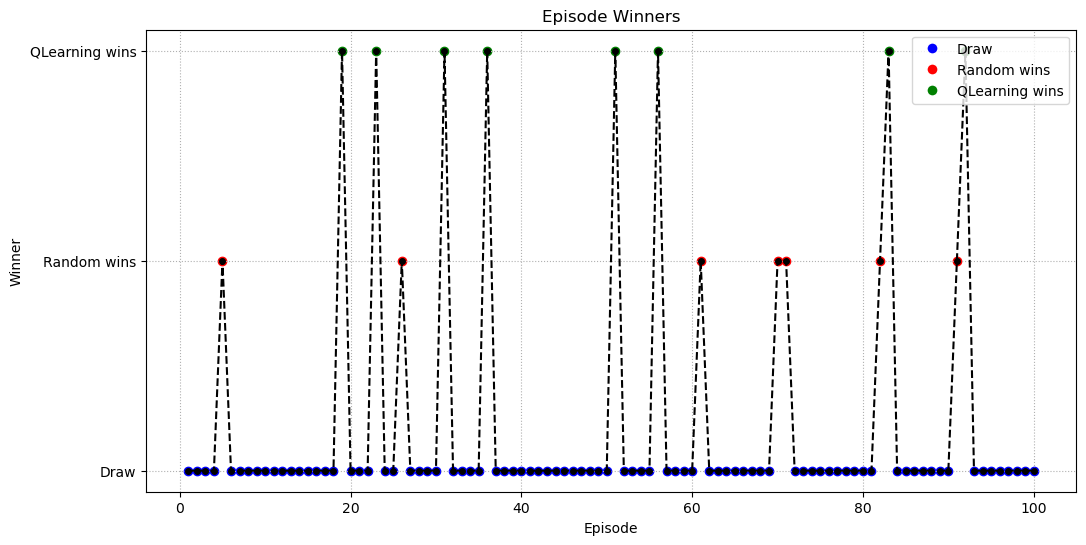
\includegraphics[width=1.2\textwidth]{img 9.png}
    \caption{Minimax vs Random Agent}
    \label{fig:example}
\end{figure}



\section{Results}

\subsection{Tic Tac Toe Game}

\begin{itemize}
  \item Minimax vs. QLearning: Minimax won all the games.
  \item Minimax vs. Random Agent: Minimax won all the games.
  \item QLearning vs. Random Agent: Initially, they were winning randomly, but QLearning started to win more once it learned.
\end{itemize}

\subsection{Connecting Four}

\begin{itemize}
  \item Minimax vs. QLearning: Minimax was winning most of the games initially, then QLearning started to learn but still couldn't defeat it.
  \item Minimax vs. Random Agent: Minimax won all the games.
  \item QLearning vs. Random Agent: Initially, they were winning randomly, but QLearning started to win more once it learned.
\end{itemize}

\subsection{Chess}

\begin{itemize}
  \item Minimax vs. QLearning: Games landed in a draw.
  \item Minimax vs. Random Agent: Minimax won all the games.
  \item QLearning vs. Random Agent: Most games landed in a draw.
\end{itemize}


\section{Discussion}

The results obtained from the experiments provide interesting observations regarding the performance of different agents in various games.

\subsection{Tic Tac Toe Game}

In the Tic Tac Toe game, the Minimax algorithm displayed a dominant performance against both the QLearning agent and the Random agent. It consistently won all the games against both opponents. This outcome showcases the strong decision-making capabilities of the Minimax algorithm, which can effectively analyze the game state and make optimal moves to secure victory.

On the other hand, the QLearning agent initially struggled against both the Minimax and Random agents, resulting in random wins. However, as the QLearning agent learned and improved its strategy over time, it started winning more frequently against the Random agent. This observation highlights the ability of QLearning to adapt and optimize its gameplay through reinforcement learning.

\subsection{Connecting Four}

In the Connecting Four game, the Minimax algorithm again demonstrated its superior performance. It consistently won all the games against both the QLearning agent and the Random agent. This outcome reinforces the effectiveness of the Minimax algorithm in strategically planning moves to achieve victory.

Similar to the Tic Tac Toe game, the QLearning agent initially faced challenges against the Minimax agent. However, it gradually learned and refined its strategy, although it was still unable to defeat the Minimax agent consistently. This observation suggests that while QLearning can learn and improve its gameplay, it may require further training or advanced techniques to surpass the performance of traditional algorithms like Minimax.

\subsection{Chess}

In the Chess games, the Minimax algorithm and the QLearning agent mostly resulted in draws when pitted against each other. This outcome indicates a balanced performance between the two opponents, where neither agent could gain a significant advantage over the other. Chess being a complex and strategic game, this result showcases the competitive nature of both Minimax and QLearning in making optimal moves.

Once again, the Minimax agent showcased its strength by winning all the games against the Random agent. This result emphasizes the robust decision-making capability of the Minimax algorithm, even when facing opponents with random move selections.

In the case of the QLearning agent against the Random agent, most games ended in draws. This outcome suggests that the QLearning agent was able to effectively respond to the Random agent's random moves, resulting in balanced gameplay.

Overall, these observations highlight the strengths and limitations of different AI agents in various game scenarios. The Minimax algorithm excels in strategic decision-making, while QLearning demonstrates adaptability and learning capabilities. Further exploration and optimization techniques can potentially enhance the performance of these agents in their respective games.


\section{Conclusion}

The experiments conducted on different AI agents in Tic Tac Toe, Connecting Four, and Chess games provide valuable insights into their performance and capabilities. Here, we summarize the key findings and draw conclusions:

The Minimax algorithm consistently demonstrated strong decision-making capabilities and strategic planning, resulting in victories against both the QLearning agent and the Random agent in all three games. Its ability to analyze game states and make optimal moves showcases its effectiveness in adversarial game scenarios.

The QLearning agent showcased its adaptability and learning capabilities by gradually improving its performance over time. It initially struggled against the Minimax algorithm but started winning more frequently against the Random agent once it learned and optimized its strategy. This highlights the potential of reinforcement learning algorithms like QLearning to adapt to changing environments and optimize gameplay through experience.

In the Chess games, both the Minimax algorithm and the QLearning agent mostly resulted in draws when playing against each other. This showcases the competitive nature of these agents in a complex and strategic game environment. Against the Random agent, the Minimax algorithm consistently emerged as the winner, highlighting its robust decision-making even against opponents with random moves. The QLearning agent achieved balanced gameplay against the Random agent, indicating its ability to effectively respond to unpredictable opponents.

Overall, the experiments provide valuable insights into the strengths and limitations of different AI agents in game scenarios. The Minimax algorithm excels in strategic planning and decision-making, while QLearning demonstrates adaptability and the potential for learning and improvement. Further research and optimization techniques can enhance the performance of these agents and extend their applicability to other complex game environments.

These findings contribute to the advancement of AI in gaming and provide a foundation for exploring more sophisticated algorithms and strategies in the future. By leveraging the strengths of different AI approaches, we can continue to push the boundaries of game-playing AI and its applications in various domains.


\section{Future Work}
The outcomes and observations obtained from the experiments provide a solid foundation for further analysis and exploration of AI agents in game scenarios. To delve deeper into understanding the reasons behind some of the observed outcomes and to enhance the performance of the agents, several avenues for future work can be explored.

Firstly, a more in-depth analysis of the decision-making process of the Minimax algorithm can be undertaken. By studying its search tree and evaluating the quality of its heuristic function, researchers can gain insights into the algorithm's performance and potentially improve its efficiency. Exploring different pruning techniques such as alpha-beta pruning or advanced heuristics can be promising directions to optimize the Minimax algorithm further.

For the QLearning agent, additional investigations can be conducted to analyze its learning process and performance. Fine-tuning the hyperparameters, such as the learning rate, discount factor, and exploration rate, may lead to improved convergence and more effective decision-making. Additionally, alternative reinforcement learning algorithms, such as Deep Q-Networks (DQN) or Monte Carlo Tree Search (MCTS), can be explored to compare their performance against QLearning in game environments.

Furthermore, studying the performance of AI agents against human players can provide valuable insights into their practical applicability. Conducting user studies and gathering feedback from human participants can help evaluate the agents' gameplay experience, identify potential biases or limitations, and guide further improvements.

To extend the analysis beyond the presented games, investigating more complex and diverse game environments can be pursued. Games with larger state and action spaces, hidden information, or simultaneous moves can pose new challenges for AI agents. Exploring advanced techniques such as deep learning-based approaches, ensemble methods, or meta-learning can enhance the agents' abilities to handle complex game dynamics and strategic decision-making.

Overall, the future work outlined here aims to provide a deeper understanding of AI agents' performance in game scenarios, improve their decision-making capabilities, and expand their applications to more challenging domains. By pushing the boundaries of AI in gaming, we can unravel new insights and pave the way for advancements in AI research and its practical applications.

\section{References}
\begin{enumerate}
    \item Sutton, R. S., \& Barto, A. G. (2018). \textit{Reinforcement Learning: An Introduction.} MIT Press.
    
    \item Russell, S. J., \& Norvig, P. (2016). \textit{Artificial Intelligence: A Modern Approach.} Pearson.
    
    \item Littman, M. L. (1994). Markov games as a framework for multi-agent reinforcement learning. In \textit{Machine Learning Proceedings 1994} (pp. 157-163).
    
    \item Silver, D., et al. (2016). Mastering the game of Go with deep neural networks and tree search. \textit{Nature, 529}(7587), 484-489.
    
    \item Tesauro, G. (1995). Temporal difference learning and TD-Gammon. \textit{Communications of the ACM, 38}(3), 58-68.
    
    \item Browne, C., et al. (2012). A survey of Monte Carlo tree search methods. \textit{IEEE Transactions on Computational Intelligence and AI in Games, 4}(1), 1-43.
    
    \item Sutton, R. S., et al. (1999). Between MDPs and semi-MDPs: A framework for temporal abstraction in reinforcement learning. \textit{Artificial Intelligence, 112}(1-2), 181-211.
    
    \item Kaelbling, L. P., et al. (1996). Reinforcement learning: A survey. \textit{Journal of Artificial Intelligence Research, 4}, 237-285.
    
    \item Mnih, V., et al. (2015). Human-level control through deep reinforcement learning. \textit{Nature, 518}(7540), 529-533.
    
    \item Busoniu, L., et al. (2010). A comprehensive survey of multiagent reinforcement learning. \textit{IEEE Transactions on Systems, Man, and Cybernetics, Part C (Applications and Reviews), 40}(6), 561-582.
    
\end{enumerate}

\end{document}
